\chapter{Referencial Teórico}
\label{cap:referencial_teorico}

%-----------------------------------
\section{Energia Solar Fotovoltaica e Eficiência Energética}
\label{sec:energia_solar}

A energia solar fotovoltaica consiste na conversão direta da radiação solar em energia elétrica por meio do efeito fotovoltaico. Esse fenômeno representa o princípio de funcionamento dos sistemas fotovoltaicos e constitui uma das principais tecnologias empregadas para o aproveitamento da energia solar.

O efeito fotovoltaico corresponde ao processo de conversão da radiação eletromagnética em energia elétrica. Nesse contexto, a radiação solar incidente sobre a superfície terrestre pode ser convertida diretamente em eletricidade por meio de sistemas fotovoltaicos \cite{olivati2001}. Quando os fótons emitidos pelo Sol incidem sobre uma célula fotovoltaica, ocorre a excitação dos elétrons presentes na estrutura do material semicondutor, geralmente o silício. Esse processo promove a movimentação desses elétrons, resultando no surgimento de uma diferença de potencial elétrico entre as extremidades da célula.

Essa diferença de potencial é consequência da existência de um campo elétrico interno formado na junção entre materiais semicondutores do tipo P e do tipo N. Como resultado, estabelece-se um fluxo ordenado de elétrons, caracterizando a corrente elétrica produzida pela célula fotovoltaica. A Figura~\ref{fig:efeito_fotovoltaico} apresenta, de forma esquemática, o princípio de funcionamento do efeito fotovoltaico, destacando a incidência da radiação solar sobre a célula, a junção PN e o deslocamento dos elétrons responsáveis pela geração da corrente elétrica.

\begin{figure}[H]
\centering
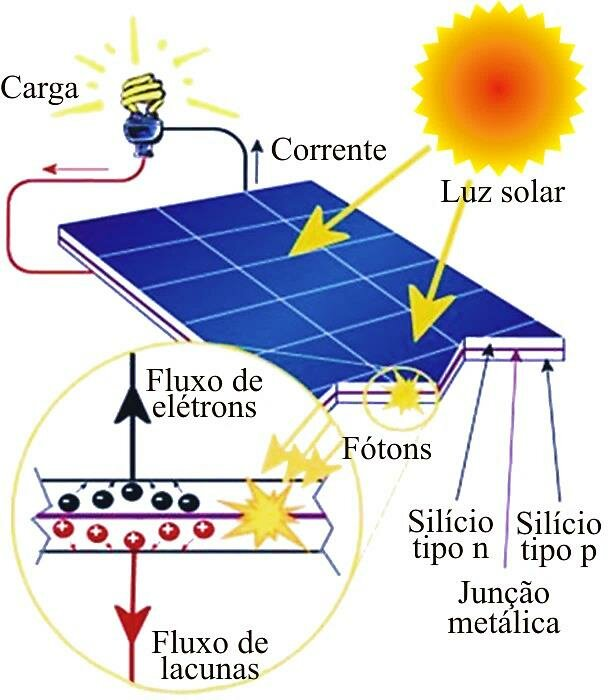
\includegraphics[width=0.70\textwidth]{Figuras/efeito_fotovoltaico.png}
\caption{Representação esquemática do efeito fotovoltaico em uma célula solar.}
\label{fig:efeito_fotovoltaico}
\fonte{Adaptado de Olivati (2001).}
\end{figure}

As células fotovoltaicas são interligadas eletricamente para formar os módulos fotovoltaicos, que constituem a unidade básica dos sistemas de geração de energia solar. O desempenho desses sistemas depende da capacidade dos módulos em converter a energia proveniente da radiação solar em energia elétrica útil. Entretanto, essa conversão é influenciada por diversos fatores, entre os quais destacam-se a irradiância solar, a temperatura de operação das células, o sombreamento, as características construtivas dos módulos, sua orientação, inclinação e o ângulo de incidência da radiação solar sobre sua superfície.

Segundo Veríssimo et al. (\citeyear{verissimo2017}), a incidência da radiação solar sobre os módulos fotovoltaicos exerce influência direta na geração de energia elétrica. Em sistemas convencionais, os painéis permanecem instalados em posição fixa, normalmente definida para maximizar a captação média anual de energia. Entretanto, como a posição aparente do Sol varia continuamente ao longo do dia, o ângulo de incidência da radiação modifica-se constantemente, fazendo com que os raios solares atinjam a superfície do painel em condições diferentes da orientação ideal durante grande parte do período de insolação.

Essa variação angular reduz a quantidade de radiação efetivamente aproveitada pelos módulos e, consequentemente, diminui a energia elétrica gerada. Dessa forma, parte das perdas observadas em sistemas fotovoltaicos não está associada apenas às características construtivas dos módulos, mas também às condições de posicionamento em relação ao Sol.

Além da orientação do painel, outros fatores também influenciam a eficiência energética do sistema, como o aumento da temperatura das células fotovoltaicas, o acúmulo de sujeira sobre os módulos, sombreamentos parciais, perdas elétricas em cabos e equipamentos de conversão de energia, bem como condições atmosféricas adversas. A atuação conjunta desses fatores pode reduzir significativamente o desempenho do sistema fotovoltaico.

Entre os fatores mencionados, a orientação do módulo em relação à radiação solar destaca-se por ser uma variável passível de controle por meio de sistemas de posicionamento automatizado. Conforme discutido por Veríssimo et al. (\citeyear{verissimo2017}), manter a incidência da radiação solar próxima da condição perpendicular ao painel favorece o aumento da energia captada, reduzindo perdas decorrentes da variação da posição aparente do Sol ao longo do dia.

Nesse contexto, a literatura apresenta diferentes estratégias para aumentar o aproveitamento energético dos sistemas fotovoltaicos, entre as quais se destacam os sistemas de rastreamento solar, responsáveis por ajustar continuamente a orientação dos módulos durante o período de operação. Os princípios de funcionamento desses sistemas serão apresentados na Seção~2.2.

%-----------------------------------
\section{Sistemas de Rastreamento Solar (Trackers)}

Embora seja a Terra que realize os movimentos de rotação e translação, para um observador localizado em sua superfície o Sol aparenta deslocar-se de leste para oeste ao longo do dia. Esse fenômeno, conhecido como movimento aparente do Sol, ocorre em decorrência da rotação terrestre. Além da variação diária, a trajetória aparente do Sol também se altera ao longo do ano devido à inclinação aproximada de 23,5° do eixo de rotação da Terra em relação ao plano de sua órbita, modificando a altura aparente do Sol e os ângulos de incidência da radiação solar sobre a superfície terrestre \cite{adolpho2024}.

A posição aparente do Sol pode ser descrita por dois parâmetros geométricos fundamentais: o ângulo de azimute solar e o ângulo de elevação solar. O ângulo de azimute representa a posição horizontal do Sol em relação aos pontos cardeais, enquanto o ângulo de elevação, também denominado altitude solar, corresponde à altura aparente do Sol acima da linha do horizonte. Esses parâmetros são amplamente utilizados na determinação da orientação de módulos fotovoltaicos e no desenvolvimento de sistemas de rastreamento solar, pois permitem estimar a direção de incidência da radiação solar ao longo do dia.

A Figura~\ref{fig:azimute} apresenta a geometria desses ângulos, ilustrando a relação entre a trajetória aparente do Sol, o ângulo de azimute e o ângulo de elevação.

\begin{figure}[H]
    \centering
    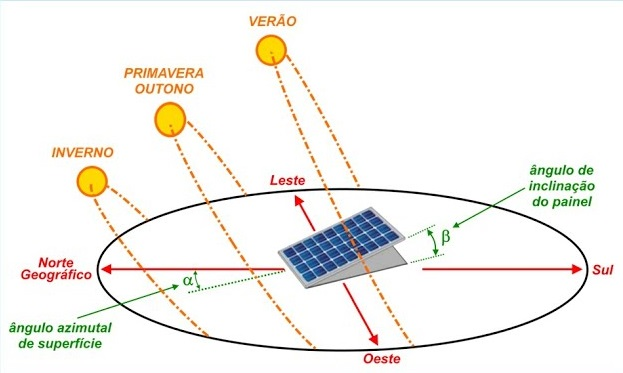
\includegraphics[width=0.75\textwidth]{Figuras/azimute_solar.jpg}
    \caption{Geometria solar ilustrando os ângulos de azimute e elevação solar.}
    \label{fig:azimute}
    \fonte{Adaptado de Adolpho Eletricista (2025).}
\end{figure}

O ângulo de azimute corresponde ao deslocamento horizontal da posição aparente do Sol em relação ao norte geográfico, sendo medido sobre o plano horizontal. Ao longo do dia, esse ângulo varia continuamente devido ao movimento aparente do Sol no sentido leste-oeste, sendo um parâmetro importante para definir a orientação horizontal de sistemas fotovoltaicos com rastreamento solar.

O ângulo de elevação solar corresponde ao ângulo formado entre a direção dos raios solares e o plano horizontal. Seu valor é aproximadamente igual a $0^\circ$ durante o nascer e o pôr do Sol, aumentando gradativamente ao longo da manhã até atingir o valor máximo nas proximidades do meio-dia solar, quando o Sol alcança sua maior altura aparente no céu. Em seguida, esse ângulo diminui progressivamente até retornar a aproximadamente $0^\circ$ no pôr do Sol.

Neste trabalho, esses conceitos são apresentados como fundamentação teórica para a compreensão do movimento aparente do Sol. Entretanto, o sistema desenvolvido utiliza como referência principal o horário para estimar a posição do painel fotovoltaico ao longo do dia, realizando posteriormente pequenos ajustes angulares com base na potência elétrica medida, sem efetuar o cálculo direto dos ângulos de azimute e elevação solar.

Na região Norte de Minas Gerais, situada aproximadamente na latitude de 16$^\circ$ Sul, observa-se elevada disponibilidade de radiação solar ao longo de praticamente todo o ano. Nessa região, a principal variação diária da posição aparente do Sol ocorre no sentido leste-oeste, associada à variação do ângulo de azimute, enquanto as alterações na elevação solar ao longo das estações do ano são relativamente menores quando comparadas às observadas em regiões de latitudes mais elevadas \cite{cemig2017}. Dessa forma, um sistema de rastreamento de eixo único, responsável por acompanhar o movimento diário do Sol no sentido leste-oeste, é capaz de proporcionar ganhos significativos na captação da radiação solar, justificando sua adoção neste trabalho.

O desempenho dos sistemas fotovoltaicos depende diretamente da quantidade de radiação solar incidente sobre a superfície dos módulos. Como os ângulos de azimute e elevação variam continuamente durante o dia e ao longo do ano, painéis instalados em posição fixa deixam de receber a radiação em condições próximas da perpendicularidade durante grande parte do período de insolação, reduzindo o aproveitamento da energia disponível.

Uma alternativa para minimizar essas perdas consiste na utilização de sistemas de rastreamento solar, também conhecidos como \textit{solar trackers}. Esses sistemas ajustam automaticamente a orientação dos módulos fotovoltaicos ao longo do dia, buscando manter a incidência da radiação solar em condições mais favoráveis e, consequentemente, aumentar a geração de energia elétrica \cite{verissimo2017}.

O princípio de funcionamento desses sistemas baseia-se no acompanhamento do movimento aparente do Sol. Esse acompanhamento pode ser realizado por diferentes estratégias, como sensores de luminosidade, modelos astronômicos baseados na posição solar ou algoritmos computacionais previamente programados. Independentemente da estratégia adotada, o objetivo permanece o mesmo: ajustar continuamente a posição do painel fotovoltaico para reduzir as perdas provocadas pela variação do ângulo de incidência da radiação solar.

Os sistemas de rastreamento podem ser classificados, de forma geral, em rastreadores de eixo único e rastreadores de dois eixos. Os rastreadores de eixo único realizam a movimentação do painel em apenas um plano, normalmente acompanhando o deslocamento do Sol no sentido leste-oeste. Em razão de sua construção mais simples, apresentam menor custo de implementação, menor consumo de energia para acionamento e menores exigências de manutenção quando comparados aos sistemas de dois eixos.

Por sua vez, os rastreadores de dois eixos permitem o movimento simultâneo em dois planos, acompanhando tanto a variação do azimute quanto da elevação solar ao longo do dia e das estações do ano. Essa configuração proporciona um alinhamento mais preciso entre o painel e a posição aparente do Sol, aumentando o aproveitamento da radiação incidente. Entretanto, apresenta maior complexidade mecânica, maior custo de fabricação, maior consumo de energia e maiores exigências de manutenção, fatores que podem limitar sua aplicação em sistemas fotovoltaicos de pequeno porte.

Diversos estudos têm demonstrado que a utilização de sistemas de rastreamento solar pode proporcionar ganhos significativos na geração de energia elétrica quando comparados aos sistemas convencionais de painel fixo. Entretanto, os resultados dependem da localização geográfica, das condições climáticas, da tecnologia empregada, do tipo de rastreador utilizado e da estratégia de controle adotada.

Nesse contexto, Almeida (\citeyear{almeida2024}) desenvolveu um sistema de rastreamento solar horizontal de eixo único utilizando o microcontrolador ESP32 como unidade de controle. O estudo propôs a substituição de controladores industriais por uma plataforma embarcada de menor custo, preservando as funcionalidades necessárias ao posicionamento automático do painel fotovoltaico. Os resultados experimentais demonstraram ganhos de geração de energia entre 17,51\% e 30,42\% em comparação com um sistema de painel fixo, indicando que rastreadores solares de eixo único representam uma alternativa tecnicamente viável para aplicações fotovoltaicas.

De forma semelhante, Moraes et al. (\citeyear{moraes2024}) avaliaram o desempenho de um sistema fotovoltaico equipado com rastreamento solar controlado por ESP32 em comparação com um sistema convencional de painel fixo. Os resultados evidenciaram um ganho energético aproximado de 37,9\%, atribuído ao melhor aproveitamento da radiação solar proporcionado pelo ajuste contínuo da orientação do painel. Além disso, o estudo destacou o potencial das plataformas embarcadas de baixo custo para o desenvolvimento de sistemas automatizados destinados à otimização da geração de energia fotovoltaica.

Os resultados apresentados nesses estudos demonstram que a utilização de rastreadores solares pode proporcionar ganhos significativos na geração de energia elétrica. Entretanto, o desempenho desses sistemas não depende apenas da estratégia de controle empregada, mas também da confiabilidade da estrutura eletromecânica responsável pelo posicionamento do painel. Motores, engrenagens e mecanismos de transmissão estão sujeitos a desgaste, desalinhamentos, falhas de acionamento e à ação de fatores ambientais, como vento, poeira e umidade. Essas condições podem comprometer o funcionamento do rastreador, mantendo o painel em posições desfavoráveis por longos períodos e reduzindo significativamente a geração de energia.

Além dos aspectos mecânicos, a confiabilidade operacional também está relacionada à arquitetura do sistema embarcado responsável pelo controle do rastreador. Sistemas baseados em microcontroladores permitem implementar algoritmos de posicionamento, controlar o acionamento dos atuadores, registrar dados de operação e integrar sensores para monitoramento do sistema. Essas funcionalidades contribuem para aumentar a robustez do sistema, reduzir movimentações desnecessárias e fornecer informações que podem ser utilizadas na identificação de falhas e na avaliação do desempenho operacional.

Nesse contexto, a utilização de modelos computacionais representa uma importante ferramenta para o desenvolvimento e a análise de sistemas de rastreamento solar. As simulações permitem avaliar diferentes estratégias de controle, estimar o comportamento do sistema em condições variadas de operação e prever seu desempenho antes da implementação física. Entretanto, para que esses modelos possam ser utilizados com confiabilidade, torna-se necessária sua validação por meio da comparação entre resultados simulados e dados experimentais obtidos em sistemas reais. Os fundamentos relacionados à modelagem e à simulação computacional são apresentados na Seção~2.4.

%-----------------------------------
\section{Sistemas Embarcados}


Os sistemas embarcados são sistemas computacionais desenvolvidos para executar funções específicas de monitoramento, controle e processamento de informações em dispositivos eletrônicos. Diferentemente dos computadores de propósito geral, esses sistemas são projetados para desempenhar tarefas dedicadas, normalmente operando em tempo real e sob restrições de processamento, consumo de energia, memória e custo de implementação.

Segundo Chase e Almeida (\citeyear{chase2007}), um sistema embarcado caracteriza-se pela integração entre hardware e software, sendo projetado para executar funções específicas. Nesse contexto, o software embarcado processa informações provenientes de sensores, executa algoritmos de controle e aciona atuadores, permitindo que o sistema responda automaticamente às condições observadas no ambiente.

De forma geral, a arquitetura de um sistema embarcado é composta por sensores responsáveis pela aquisição de dados do ambiente, um microcontrolador encarregado do processamento dessas informações e atuadores que executam as ações determinadas pelo algoritmo de controle. A Figura~\ref{fig:embarcado} apresenta, de forma simplificada, o funcionamento básico de um sistema embarcado, destacando a interação entre o ambiente, os dispositivos de entrada e saída e a unidade de processamento.

\begin{figure}[H]
    \centering
    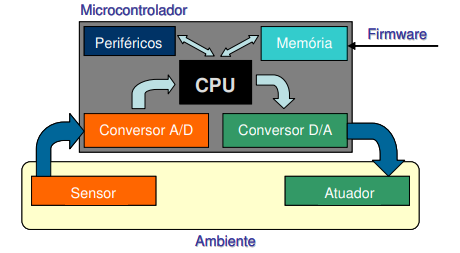
\includegraphics[width=0.85\textwidth]{Figuras/sistemas_embarcados.png}
    \caption{Diagrama básico de um sistema embarcado dotado de um microcontrolador monitorando o ambiente.}
    \label{fig:embarcado}
    \fonte{Adaptado de Chase e Almeida (2007).}
\end{figure}

Essa arquitetura é amplamente empregada em aplicações de automação industrial, robótica, Internet das Coisas (IoT), sistemas automotivos e monitoramento remoto. No contexto deste trabalho, esse modelo é aplicado ao sistema fotovoltaico automatizado, no qual o microcontrolador realiza a aquisição de dados provenientes dos sensores, processa as informações e controla o posicionamento do painel fotovoltaico por meio de um atuador.

O microcontrolador constitui o elemento central dessa arquitetura, sendo responsável pela execução do algoritmo de controle, pela leitura dos sinais provenientes dos sensores e pelo acionamento dos dispositivos de saída. Dessa forma, integra aquisição de dados, processamento e tomada de decisão em tempo real, permitindo que o sistema opere de maneira autônoma e responda às condições de funcionamento previamente estabelecidas.

Diversas plataformas baseadas em microcontroladores são empregadas no desenvolvimento de sistemas embarcados, destacando-se dispositivos das famílias PIC, AVR, ESP32, STM32 e Raspberry Pi Pico. A escolha da plataforma depende dos requisitos da aplicação, considerando fatores como capacidade de processamento, memória disponível, número de entradas e saídas, interfaces de comunicação, consumo de energia e custo de implementação.

Para aplicações de automação em sistemas fotovoltaicos de pequeno porte, plataformas baseadas na arquitetura AVR, como o Arduino Uno, apresentam capacidade computacional suficiente para executar algoritmos de controle, realizar a aquisição de dados provenientes de sensores e acionar dispositivos eletromecânicos. Além disso, a ampla disponibilidade de bibliotecas, interfaces de comunicação e módulos compatíveis favorece sua utilização em pesquisas experimentais e no desenvolvimento de protótipos acadêmicos \cite{arduino2023}.

Os sensores constituem a interface entre o ambiente físico e o sistema computacional, convertendo grandezas físicas em sinais elétricos interpretáveis pelo microcontrolador. Em sistemas fotovoltaicos, esses dispositivos permitem monitorar continuamente variáveis como tensão, corrente, temperatura e irradiância, fornecendo informações essenciais para a avaliação do desempenho energético e para a implementação de estratégias de controle.

Os atuadores são responsáveis por converter os comandos emitidos pelo sistema de controle em ações físicas sobre o processo monitorado. Em sistemas fotovoltaicos automatizados, essa função consiste em movimentar mecanicamente o painel fotovoltaico conforme a estratégia de posicionamento definida pelo algoritmo de controle. Entre os dispositivos mais utilizados em aplicações experimentais destacam-se os servomotores, que permitem o controle preciso da posição angular por meio de sinais PWM (\textit{Pulse Width Modulation}), apresentando boa precisão de posicionamento, simplicidade de integração e reduzida complexidade de controle \cite{arduino2023} .

Além dos elementos principais, sistemas embarcados frequentemente incorporam módulos auxiliares destinados ao armazenamento de dados, sincronização temporal e interface com o usuário. Dispositivos como módulos de cartão SD, relógios de tempo real (RTC) e displays permitem registrar informações experimentais, manter a referência temporal das medições e acompanhar o funcionamento do sistema durante sua operação.

A integração entre sensores, microcontroladores, atuadores e módulos auxiliares constitui a base dos sistemas embarcados modernos, possibilitando a aquisição contínua de dados, o processamento em tempo real, o controle automático de processos físicos e o armazenamento das informações produzidas. Essas características tornam essa arquitetura adequada para aplicações de automação, monitoramento e controle, incluindo sistemas fotovoltaicos automatizados.
%-----------------------------------
\section{Modelagem e Simulação de Sistemas}

A modelagem computacional consiste na representação matemática de sistemas físicos com o objetivo de descrever e prever seu comportamento por meio de modelos capazes de reproduzir, de forma aproximada, os fenômenos observados na realidade. Associada à simulação computacional, essa abordagem permite analisar diferentes condições de operação sem a necessidade da construção imediata de protótipos físicos, reduzindo tempo, custos de desenvolvimento e riscos experimentais \cite{dvorak2023}.

Segundo Melo (\citeyear{melo2019}), a determinação da posição aparente do Sol por meio de parâmetros astronômicos constitui a base para modelos computacionais empregados na simulação do desempenho de sistemas fotovoltaicos. Esses modelos possibilitam estimar o comportamento do sistema sob diferentes condições de operação, servindo como ferramenta de apoio ao projeto e à análise de desempenho.

Entre as ferramentas utilizadas para modelagem de sistemas destaca-se o \textit{MATrix LABoratory} (MATLAB) e seu ambiente de simulação Simulink, amplamente empregados em aplicações de engenharia devido à disponibilidade de bibliotecas para modelagem matemática, processamento numérico e simulação de sistemas dinâmicos. O Simulink permite representar modelos por meio de diagramas de blocos, facilitando a implementação de sistemas de controle e a análise do comportamento de processos físicos \cite{mathworks_simulink}.

Neste trabalho foi adotado como ponto de partida o modelo computacional disponibilizado por Nagi (\citeyear{nagi2023}), implementado no ambiente MATLAB/Simulink para comparação entre sistemas fotovoltaicos com painel fixo e com rastreamento solar. O modelo foi adaptado para representar as características do sistema automatizado desenvolvido nesta pesquisa e posteriormente validado por meio da comparação entre os resultados simulados e os dados experimentais obtidos com o protótipo físico.

Embora a modelagem computacional permita analisar previamente o comportamento do sistema, sua confiabilidade depende da capacidade do modelo em representar adequadamente o sistema físico. Dessa forma, a validação experimental constitui uma etapa essencial do processo de modelagem, sendo realizada por meio da comparação entre os resultados simulados e os dados obtidos experimentalmente em condições equivalentes de operação \cite{dvorak2023}. Essa comparação permite verificar a representatividade do modelo computacional em relação ao comportamento observado na prática, aumentando sua confiabilidade para análises e estudos futuros.

A utilização conjunta da modelagem computacional e da experimentação física constitui uma estratégia importante para o desenvolvimento de sistemas fotovoltaicos automatizados. Enquanto o modelo computacional possibilita prever o comportamento esperado do sistema em diferentes condições de operação, os ensaios experimentais permitem verificar sua representatividade em condições reais. Dessa forma, a comparação entre simulação e experimento fornece evidências sobre a validade do modelo computacional e amplia sua confiabilidade como ferramenta de apoio ao desenvolvimento e à avaliação de sistemas fotovoltaicos automatizados.